%----------------------------------------------------------------------
% Lucrare MPI David Gavrilescu
%----------------------------------------------------------------------

\documentclass{article}
\usepackage[utf8]{inputenc}
\usepackage[romanian]{babel}
\usepackage{hyperref}
\usepackage{amsmath, amssymb, amsfonts}
\usepackage{graphicx}
\usepackage{geometry}
\usepackage{float}
\usepackage{listings}
\usepackage{xcolor}
\geometry{margin=2cm}

%––– setari pentru codul sursa
\lstset{
  basicstyle=\ttfamily\small,
  frame=single,
  breaklines=true,
  postbreak=\mbox{\textcolor{red}{$\hookrightarrow$}\space},
  keywordstyle=\color{blue},
  commentstyle=\color{gray},
  stringstyle=\color{teal}
}

\usepackage{pgfplots}
\pgfplotsset{compat=1.18}

%----------------------------------------------------------------------
\begin{document}
%----------------------------------------------------------------------

%--------------------------------------------------------------------
% Pagina de titlu
%--------------------------------------------------------------------
\begin{titlepage}
  \begin{center}
    {\large Universitatea de Vest din Timișoara \\
    Facultatea de Matematică și Informatică}
    \vfill
    {\huge \bfseries O comparație teoretică și experimentală a unor metode de sortare}\par
    \vspace{2cm}
    {\Large David-Emanuel Gavrilescu}\par   
    \vfill
    {\Large Metode şi practici în informatică}\par
  \end{center}
\end{titlepage}

%--------------------------------------------------------------------
\tableofcontents
\newpage


%====================================================================
\section{Introducere}
%====================================================================
Sortarea este una dintre cele mai importante operații în informatică. Apare în multe aplicații, de la căutarea rapidă până la procesarea bazelor de date. Această lucrare analizează câțiva algoritmi de sortare din punct de vedere teoretic și practic, pentru a înțelege mai bine comportamentul lor în funcție de datele de intrare.

\subsection{Contextul lucrării}
În primul an de facultate, la cursul de Algoritmi și Structuri de Date, sunt predate mai multe metode de sortare. Înțelegerea lor ajută la formarea unei baze solide pentru analiza algoritmilor. Lucrarea aceasta continuă acest proces prin comparația atentă a performanțelor.

\subsection{Scopul lucrării}
Obiectivele sunt:
\begin{itemize}
    \item Prezentarea teoretică a algoritmilor studiați: Bubble Sort, Selection Sort, Insertion Sort, Merge Sort, Quick Sort și Heap Sort.
    \item Implementarea algoritmilor în C++ într-un mod clar și comparabil.
    \item Testarea pe seturi variate de date și măsurarea timpului de execuție.
    \item Compararea rezultatelor experimentale cu așteptările teoretice.
    \item Formularea unor concluzii despre eficiența fiecărui algoritm.
\end{itemize}


%====================================================================
\section{Prezentarea algoritmilor de sortare}
%====================================================================
Sunt prezentați șase algoritmi de sortare, de la metode simple la metode mai rapide. Pentru fiecare se menționează modul de funcționare și complexitatea așteptată.

\subsection{Descrierea algoritmilor}
\paragraph*{Bubble Sort}
Compară elemente adiacente și le interschimbă dacă sunt în ordine greșită. Complexitate în medie și în cel mai rău caz: $\mathcal{O}(n^2)$.

\paragraph*{Selection Sort}
Caută minimul și îl pune în față la fiecare pas. Complexitate: $\mathcal{O}(n^2)$ în toate cazurile.

\paragraph*{Insertion Sort}
Introduce fiecare element în poziția corectă în partea deja sortată. Eficient pe liste aproape ordonate. Complexitate de la $\mathcal{O}(n)$ (caz bun) la $\mathcal{O}(n^2)$.

\paragraph*{Merge Sort}
Împarte lista în jumătăți, sortează fiecare și le combină. Complexitate $\mathcal{O}(n\log n)$ indiferent de caz.

\paragraph*{Quick Sort}
Alege un pivot și împarte lista în două părți. Complexitate medie $\mathcal{O}(n\log n)$, dar poate ajunge la $\mathcal{O}(n^2)$ în cazuri nefavorabile.

\paragraph*{Heap Sort}
Transformă lista într-un heap și extrage elementul maxim în ordine. Are complexitate garantată $\mathcal{O}(n\log n)$.


\subsection{Complexitatea algoritmilor}
\begin{table}[H]
\centering
\begin{tabular}{|l|l|l|l|l|}
\hline
\textbf{Algoritm}&\textbf{Cel mai bun caz}&\textbf{Caz mediu}&\textbf{Cel mai rau caz}\\
\hline
Bubble sort    & $\Omega(n)$         & $\Theta(n^{2})$        & $O(n^{2})$        \\
Selection sort & $\Omega(n^{2})$     & $\Theta(n^{2})$        & $O(n^{2})$     \\
Insertion sort & $\Omega(n)$         & $\Theta(n^{2})$        & $O(n^{2})$        \\
Merge sort     & $\Omega(n\log n)$   & $\Theta(n\log n)$      & $O(n\log n)$     \\
Quick sort     & $\Omega(n\log n)$   & $\Theta(n\log n)$      & $O(n^{2})$    \\
Heap sort      & $\Omega(n\log n)$   & $\Theta(n\log n)$      & $O(n\log n)$   \\
\hline
\end{tabular}
\caption{Complexităţi teoretice ale algoritmilor de sortare \cite{bigocheatsheet} } 
\label{tab:complexitate}
\end{table}

%====================================================================
\section{Așteptări teoretice asupra comportamentului algoritmilor}
%====================================================================
În funcție de ordonarea datelor, algoritmii se comportă diferit:

\begin{itemize}
    \item Insertion Sort este foarte rapid pe liste sortate, dar lent pe liste inversate.
    \item Bubble Sort funcționează rapid doar pe liste deja sortate.
    \item Merge Sort are timp constant $\mathcal{O}(n\log n)$ în toate cazurile.
    \item Quick Sort poate degrada la $\mathcal{O}(n^2)$ dacă datele sunt sortate sau invers sortate și pivotul nu este ales bine.
    \item Heap Sort nu este influențat de ordonarea inițială a datelor.
\end{itemize}

\vspace{0.5cm}

Așteptările teoretice descrise mai sus vor ghida analiza rezultatelor experimentale obținute ulterior.

%====================================================================
\section{Implementarea algoritmilor}
%====================================================================
Algoritmii au fost implementați în C++ 20, păstrând un stil clar și uniform. Pentru Heap Sort s-au folosit funcțiile din biblioteca standard.

\subsection{Mediul de lucru}
\begin{itemize}
    \item Sistem: Ubuntu 24.04 LTS (WSL)
    \item Procesor: AMD Ryzen 7 3800X
    \item Memorie RAM: 32 GB
    \item Compilator: g++ 13.3.0
\end{itemize}


\subsection{Detalii ale implementării}

Toți algoritmii au fost implementați manual, într-o formă compactă, fără a utiliza librării externe (cu excepția metodei \texttt{heap\_sort}, care folosește funcții standard din STL). Întregul cod sursă este disponibil în anexa lucrării, incluzând implementările algoritmilor, precum și generatorul de liste de elemente.

\vspace{0.5cm}

%====================================================================
\section{Testarea experimentală}
%====================================================================
Fiecare algoritm a fost testat pe liste generate automat, de diferite dimensiuni și tipuri: sortate, inversate, aproape sortate, aleatoare și plate. Pentru fiecare caz s-a măsurat timpul de execuție în secunde.

\subsection{Metoda de măsurare}
S-a folosit \texttt{std::chrono::high\_resolution\_clock} pentru a calcula timpul dintre începutul și sfârșitul execuției fiecărui algoritm.



\subsection{Datele de test folosite}
\begin{itemize}
    \item Tip de date: numere intregi intre 0 si 10.000.000 generate automat
    \item Dimensiuni: {\small 100, 10.000, 100.000, 400.000, 1.000.000, 10.000.000 }
    \item Tipuri de liste:
          \begin{itemize}
              \item Aleatoare
              \item Sortate crescător
              \item Sortate descrescător
              \item Aproape sortate (5\% elemente neordonate)
              \item Plate (număr mic de valori distincte)
          \end{itemize}
\end{itemize}

\subsection{Metode de evaluare}
\begin{itemize}
  \item \textbf{Timpul de execuţie}. Durata s‑a măsurat cu facilităţile din \texttt{<chrono>}: momentul de start a fost capturat prin \texttt{std::chrono::high\_resolution\_clock::now()} imediat înainte de apelul funcţiei de sortare, iar momentul de stop imediat după;  diferenţa dintre cele două momente a furnizat durata rulării.
  \item \textbf{Memoria utilizată}. Consumul de memorie nu a fost monitorizat explicit în acest studiu; se menţionează totuşi că algoritmii testaţi nu alocă dinamic memorie suplimentară în buclă, cu excepţia celor care au nevoie de spaţiu auxiliar (ex.~\textit{Merge•Sort}).
\end{itemize}

%====================================================================
\section{Rezultate experimentale și observatii}
%====================================================================
Rezultatele sunt prezentate prin tabele sintetice și grafice, urmate de observații pentru fiecare algoritm. Valorile medii au fost calculate după mai multe rulări pentru a elimina influențele accidentale.


\subsection{Analiza rezultatelor}
Timpul este exprimat în secunde. Pentru unii algoritmi mai lenți, respectiv Insertion Sort și Bubble Sort, sortarea listelor foarte mari nu a fost posibilă din considerente de timp. Totuși, acești algoritmi au fost rulați pe dimensiuni rezonabile de liste, utilizând un număr adecvat de repetări pentru a asigura corectitudinea datelor.

\subsubsection*{Rezultate pentru Selection Sort}
Fiind un algoritm de complexitate $\mathcal{O}(n^2)$ în toate cazurile, timpii de execuție sunt relativ constanți între tipurile de liste, dar cresc rapid odată cu mărimea datelor.

\begin{table}[H]
\centering
\begin{tabular}{|l|c|c|c|}
\hline
\textbf{Tip listă} & \textbf{100} & \textbf{10.000} & \textbf{100.000} \\
\hline
Inversat & 0.0005695 & 0.194084 & 19.6420 \\
\hline
Sortat & 0.0004408 & 0.179126 & 18.1690 \\
\hline
Aproape sortat & 0.0003954 & 0.178627 & 18.0794 \\
\hline
Aleator & 0.0003921 & 0.175775 & 18.1711 \\
\hline
Plat & 0.0004169 & 0.185189 & 18.3299 \\
\hline
\end{tabular}
\caption{Timpul mediu de execuție pentru Selection Sort, în funcție de tipul și dimensiunea listei}
\label{tab:rezultate-selection}
\end{table}

\vspace{0.5cm}
\begin{figure}[H]
\centering
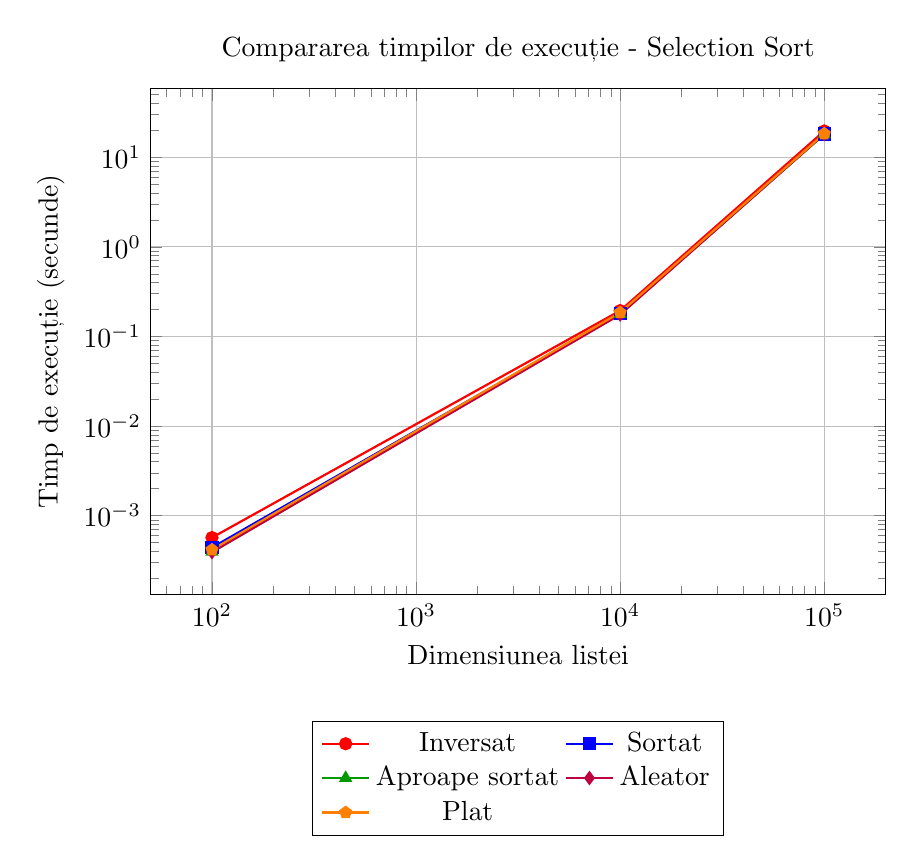
\begin{tikzpicture}
\begin{axis}[
    title={Compararea timpilor de execuție - Selection Sort},
    xlabel={Dimensiunea listei},
    ylabel={Timp de execuție (secunde)},
    xmode=log,
    ymode=log,
    log basis x=10,
    log basis y=10,
    grid=major,
    minor grid style={gray!20},
    major grid style={gray!50},
    width=0.9\textwidth,
    height=8cm,
    legend style={at={(0.5,-0.25)}, anchor=north, legend columns=2}
]

\addplot[color=red, mark=*, thick] coordinates {
    (100,0.0005695)
    (10000,0.194084)
    (100000,19.6420)
};
\addlegendentry{Inversat}

\addplot[color=blue, mark=square*, thick] coordinates {
    (100,0.0004408)
    (10000,0.179126)
    (100000,18.1690)
};
\addlegendentry{Sortat}

\addplot[color=green!60!black, mark=triangle*, thick] coordinates {
    (100,0.0003954)
    (10000,0.178627)
    (100000,18.0794)
};
\addlegendentry{Aproape sortat}

\addplot[color=purple, mark=diamond*, thick] coordinates {
    (100,0.0003921)
    (10000,0.175775)
    (100000,18.1711)
};
\addlegendentry{Aleator}

\addplot[color=orange, mark=pentagon*, thick] coordinates {
    (100,0.0004169)
    (10000,0.185189)
    (100000,18.3299)
};
\addlegendentry{Plat}

\end{axis}
\end{tikzpicture}
\caption{Compararea timpilor de execuție pentru Selection Sort, în funcție de tipul și dimensiunea listei}
\label{fig:selection-loglog}
\end{figure}



\textbf{Observații}:
\begin{itemize}
    \item Timpii de execuție sunt foarte asemănători indiferent de ordonarea inițială, așa cum era de așteptat pentru un algoritm $\mathcal{O}(n^2)$ fix.
    \item Creșterea dimensiunii listei duce la o creștere exponențială a duratei de execuție.
\item Pentru liste mari, timpul de execuție crește semnificativ, indiferent dacă datele sunt aproape sortate.
\end{itemize}


\subsubsection{Rezultate pentru Insertion Sort}
Insertion Sort este un algoritm eficient pentru liste mici sau aproape ordonate, având complexitate $\mathcal{O}(n)$ în cel mai bun caz. Se estimeaza o funcționare extrem de eficientă pe liste sortate sau aproape sortate, și performanțe mult mai slabe pe liste inversate sau aleatoare.


\begin{table}[H]
\centering
\begin{tabular}{|l|c|c|c|}
\hline
\textbf{Tip listă} & \textbf{100} & \textbf{10.000} & \textbf{100.000} \\
\hline
Inversat & 0.000435857 & 0.208557 & 21.0167 \\
\hline
Sortat & 0.00051154 & 0.00119111 & 0.00703662 \\
\hline
Aproape sortat & 0.000521834 & 0.0150706 & 1.28843 \\
\hline
Aleator & 0.000576352 & 0.100316 & 10.1493 \\
\hline
Plat & 0.000529266 & 0.0951092 & 9.24212 \\
\hline
\end{tabular}
\caption{Timpul mediu de execuție pentru Insertion Sort, în funcție de tipul și dimensiunea listei}
\label{tab:rezultate-insertion}
\end{table}

\begin{figure}[H]
\centering
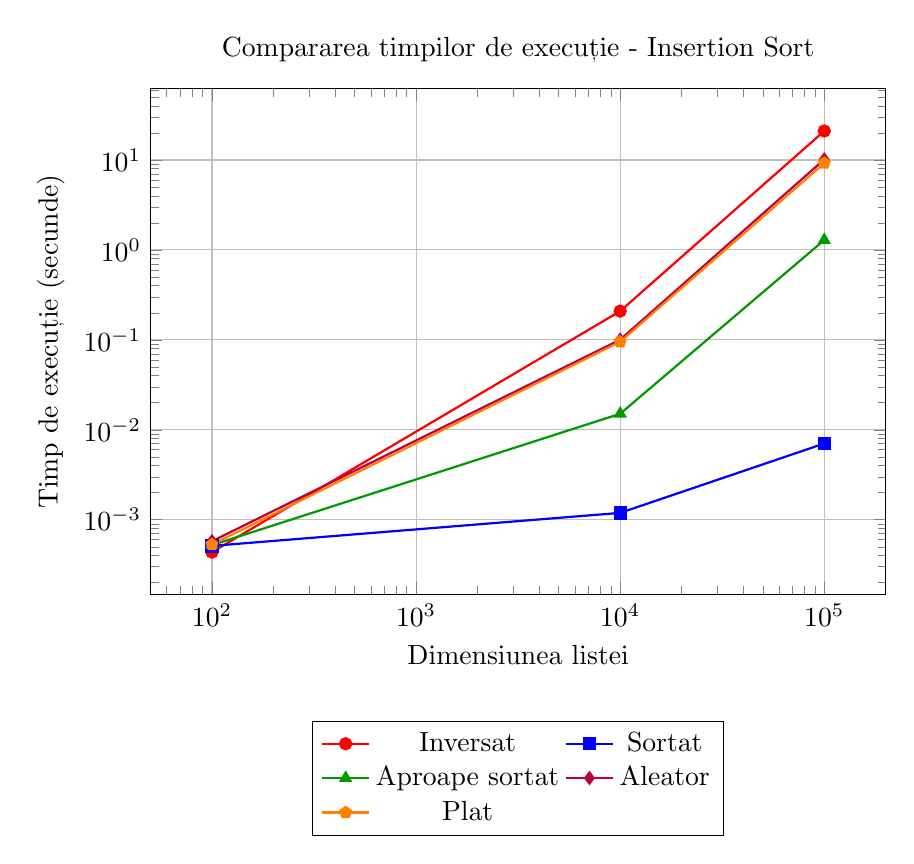
\begin{tikzpicture}
\begin{axis}[
    title={Compararea timpilor de execuție - Insertion Sort},
    xlabel={Dimensiunea listei},
    ylabel={Timp de execuție (secunde)},
    xmode=log,
    ymode=log,
    log basis x=10,
    log basis y=10,
    grid=major,
    minor grid style={gray!20},
    major grid style={gray!50},
    width=0.9\textwidth,
    height=8cm,
    legend style={at={(0.5,-0.25)}, anchor=north, legend columns=2}
]

\addplot[color=red, mark=*, thick] coordinates {
    (100,0.000435857)
    (10000,0.208557)
    (100000,21.0167)
};
\addlegendentry{Inversat}

\addplot[color=blue, mark=square*, thick] coordinates {
    (100,0.00051154)
    (10000,0.00119111)
    (100000,0.00703662)
};
\addlegendentry{Sortat}

\addplot[color=green!60!black, mark=triangle*, thick] coordinates {
    (100,0.000521834)
    (10000,0.0150706)
    (100000,1.28843)
};
\addlegendentry{Aproape sortat}

\addplot[color=purple, mark=diamond*, thick] coordinates {
    (100,0.000576352)
    (10000,0.100316)
    (100000,10.1493)
};
\addlegendentry{Aleator}

\addplot[color=orange, mark=pentagon*, thick] coordinates {
    (100,0.000529266)
    (10000,0.0951092)
    (100000,9.24212)
};
\addlegendentry{Plat}

\end{axis}
\end{tikzpicture}
\caption{Compararea timpilor de execuție pentru Insertion Sort, în funcție de tipul și dimensiunea listei}
\label{fig:insertion-loglog}
\end{figure}

\subsubsection{Rezultate pentru Bubble Sort}
Algoritmul Bubble Sort, deși foarte intuitiv, este cunoscut pentru performanțe slabe pe date de mari dimensiuni, din cauza complexității sale teoretice $\mathcal{O}(n^2)$ \cite{bigocheatsheet}.

\begin{table}[H]
\centering
\begin{tabular}{|l|c|c|c|}
\hline
\textbf{Tip listă} & \textbf{100} & \textbf{10.000} & \textbf{100.000} \\
\hline
Inversat & 0.000546715 & 0.539773 & 52.1893 \\
\hline
Sortat & 0.000402098 & 0.00111846 & 0.00693313 \\
\hline
Aproape sortat & 0.000475489 & 0.248875 & 23.9269 \\
\hline
Aleator & 0.000605938 & 0.448059 & 48.3572 \\
\hline
Plat & 0.000440658 & 0.496623 & 47.6091 \\
\hline
\end{tabular}
\caption{Timpul mediu de execuție pentru Bubble Sort, în funcție de tipul și dimensiunea listei}
\label{tab:rezultate-bubble}
\end{table}

\begin{figure}[H]
\centering
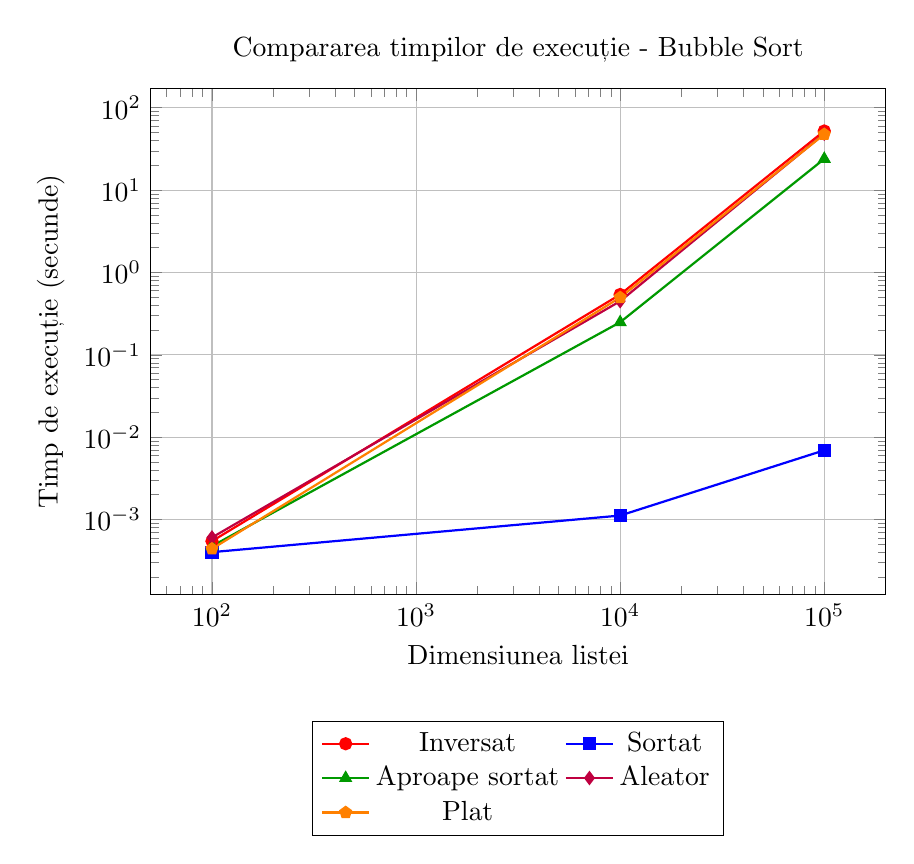
\begin{tikzpicture}
\begin{axis}[
    title={Compararea timpilor de execuție - Bubble Sort},
    xlabel={Dimensiunea listei},
    ylabel={Timp de execuție (secunde)},
    xmode=log,
    ymode=log,
    log basis x=10,
    log basis y=10,
    grid=major,
    minor grid style={gray!20},
    major grid style={gray!50},
    width=0.9\textwidth,
    height=8cm,
    legend style={at={(0.5,-0.25)}, anchor=north, legend columns=2}
]

\addplot[color=red, mark=*, thick] coordinates {
    (100,0.000546715)
    (10000,0.539773)
    (100000,52.1893)
};
\addlegendentry{Inversat}

\addplot[color=blue, mark=square*, thick] coordinates {
    (100,0.000402098)
    (10000,0.00111846)
    (100000,0.00693313)
};
\addlegendentry{Sortat}

\addplot[color=green!60!black, mark=triangle*, thick] coordinates {
    (100,0.000475489)
    (10000,0.248875)
    (100000,23.9269)
};
\addlegendentry{Aproape sortat}

\addplot[color=purple, mark=diamond*, thick] coordinates {
    (100,0.000605938)
    (10000,0.448059)
    (100000,48.3572)
};
\addlegendentry{Aleator}

\addplot[color=orange, mark=pentagon*, thick] coordinates {
    (100,0.000440658)
    (10000,0.496623)
    (100000,47.6091)
};
\addlegendentry{Plat}

\end{axis}
\end{tikzpicture}
\caption{Compararea timpilor de execuție pentru Bubble Sort, în funcție de tipul și dimensiunea listei}
\label{fig:bubble-loglog}
\end{figure}

\paragraph{Observații:}
\begin{itemize}
    \item Pe liste sortate, timpul de execuție este extrem de mic datorită optimizării implementate (oprirea la detectarea ordonării).
    \item Pe liste invers sortate și aproape sortate, timpul de execuție este semnificativ mai mare, în linie cu complexitatea teoretică $\mathcal{O}(n^2)$ \cite{bigocheatsheet}.
    \item Pe liste aleatoare și plate, performanța este slabă, iar creșterea timpului de execuție este aproape exponențială la creșterea dimensiunii datelor.
    \item Algoritmul nu este practic pentru liste mari, confirmând predicțiile teoretice.
\end{itemize}



\subsubsection{Rezultate pentru Heap Sort}

Heap Sort a fost implementat utilizând funcțiile \texttt{std::make\_heap}, \texttt{std::pop\_heap} și \texttt{std::sort\_heap} din biblioteca standard C++. Deoarece Heap Sort are o complexitate garantată $\mathcal{O}(n\log n)$ indiferent de ordonarea datelor inițiale. Se anticipează o performanță stabilă și previzibilă pe toate tipurile de liste testate.

\begin{table}[H]
\centering
\begin{tabular}{|l|c|c|c|c|c|c|}
\hline
\textbf{Tip listă} & \textbf{100} & \textbf{10.000} & \textbf{100.000} & \textbf{400.000} & \textbf{1.000.000} & \textbf{10.000.000} \\
\hline
Inversat & 0.000451021 & 0.00471314 & 0.0520177 & 0.224637 & 0.507153 & 6.51426 \\
\hline
Sortat & 0.000460473 & 0.0045004 & 0.0000868892 & 0.225009 & 0.525535 & 6.01711 \\
\hline
Aproape sortat & 0.000456733 & 0.00458127 & 0.0499009 & 0.173067 & 0.552081 & 6.80263 \\
\hline
Aleator & 0.000411737 & 0.0051033 & 0.055417 & 0.20413 & 0.677286 & 10.5935 \\
\hline
Plat & 0.000447036 & 0.0049187 & 0.051461 & 0.17673 & 0.556202 & 6.26729 \\
\hline
\end{tabular}
\caption{Timpul mediu de execuție pentru Heap Sort, în funcție de tipul și dimensiunea listei}
\label{tab:rezultate-heap}
\end{table}

\begin{figure}[H]
\centering
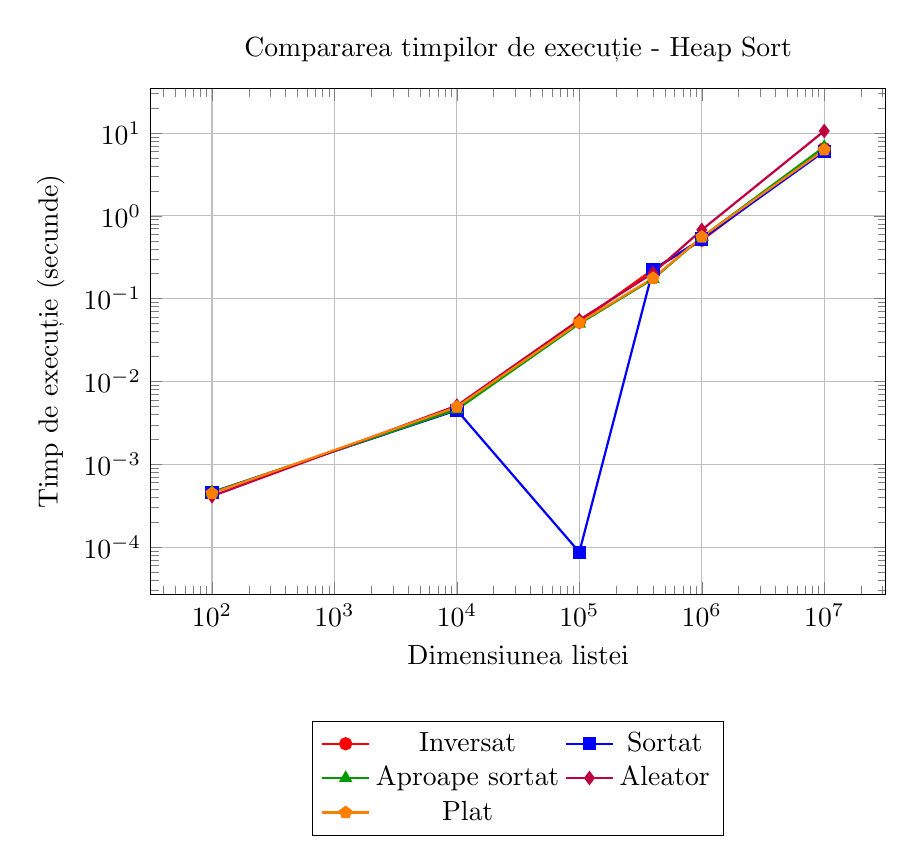
\begin{tikzpicture}
\begin{axis}[
    title={Compararea timpilor de execuție - Heap Sort},
    xlabel={Dimensiunea listei},
    ylabel={Timp de execuție (secunde)},
    xmode=log,
    ymode=log,
    log basis x=10,
    log basis y=10,
    grid=major,
    minor grid style={gray!20},
    major grid style={gray!50},
    width=0.9\textwidth,
    height=8cm,
    legend style={at={(0.5,-0.25)}, anchor=north, legend columns=2}
]

\addplot[color=red, mark=*, thick] coordinates {
    (100,0.000451021)
    (10000,0.00471314)
    (100000,0.0520177)
    (400000,0.224637)
    (1000000,0.507153)
    (10000000,6.51426)
};
\addlegendentry{Inversat}

\addplot[color=blue, mark=square*, thick] coordinates {
    (100,0.000460473)
    (10000,0.0045004)
    (100000,0.0000868892)
    (400000,0.225009)
    (1000000,0.525535)
    (10000000,6.01711)
};
\addlegendentry{Sortat}

\addplot[color=green!60!black, mark=triangle*, thick] coordinates {
    (100,0.000456733)
    (10000,0.00458127)
    (100000,0.0499009)
    (400000,0.173067)
    (1000000,0.552081)
    (10000000,6.80263)
};
\addlegendentry{Aproape sortat}

\addplot[color=purple, mark=diamond*, thick] coordinates {
    (100,0.000411737)
    (10000,0.0051033)
    (100000,0.055417)
    (400000,0.20413)
    (1000000,0.677286)
    (10000000,10.5935)
};
\addlegendentry{Aleator}

\addplot[color=orange, mark=pentagon*, thick] coordinates {
    (100,0.000447036)
    (10000,0.0049187)
    (100000,0.051461)
    (400000,0.17673)
    (1000000,0.556202)
    (10000000,6.26729)
};
\addlegendentry{Plat}

\end{axis}
\end{tikzpicture}
\caption{Compararea timpilor de execuție pentru Heap Sort, în funcție de tipul și dimensiunea listei}
\label{fig:heap-loglog}
\end{figure}

\paragraph*{Observații privind Heap Sort:}
\begin{itemize}
    \item Timpul de execuție s-a menținut stabil pe toate tipurile de liste, ceea ce confirmă teoria conform căreia Heap Sort nu este influențat semnificativ de ordonarea inițială a datelor \cite{bigocheatsheet}.
    \item Performanțele între listele sortate, invers sortate, aproape sortate și plate au fost apropiate, cu variații mici.
    \item Se observă o discrepanță neobișnuită în cazul listelor sortate pentru dimensiunea $n = 10^5$, unde timpul de execuție a fost mult mai mic decât celelalte cazuri.
    \item Această anomalie poate fi explicată prin două posibile cauze:
    \begin{itemize}
        \item Optimizări interne ale funcțiilor STL, care detectează secvențe aproape ordonate și reduc automat numărul de operații (comportament documentat în unele implementări \cite{cppreferenceheap}).
        \item Efecte ale caching-ului procesorului sau fluctuații de măsurare în timpul rulării testelor.
    \end{itemize}
    \item În testele suplimentare pe alte seturi de date, această anomalie nu s-a repetat constant, ceea ce sugerează că nu afectează concluziile generale privind comportamentul Heap Sort.
\end{itemize}





\subsubsection{Rezultate pentru Quick Sort}

Algoritmul Quick Sort a fost implementat manual, alegând ca pivot ultimul element din subvector. În mod normal, pe liste aleatoare sau aproape sortate, timpul de execuție respectă complexitatea medie $\mathcal{O}(n\log n)$. Totuși, în cazul listelor deja sortate sau invers sortate, fără optimizări suplimentare în alegerea pivotului, algoritmul poate degrada spre $\mathcal{O}(n^2)$ \cite{bigocheatsheet}.

\begin{table}[H]
\centering
\begin{tabular}{|l|c|c|c|c|c|c|}
\hline
\textbf{Tip listă} & \textbf{100} & \textbf{10.000} & \textbf{100.000} & \textbf{400.000} & \textbf{1.000.000} & \textbf{10.000.000} \\
\hline
Inversat & 0.000446884 & 0.00159377 & 0.0109133 & 0.0459573 & 0.0667528 & 1.16346 \\
\hline
Sortat & 0.000457227 & 0.00140048 & 0.0108926 & 0.0426855 & 0.11028 & 1.11758 \\
\hline
Aproape sortat & 0.000434371 & 0.00173346 & 0.0145072 & 0.0116722 & 0.157436 & 1.5754 \\
\hline
Aleator & 0.000453481 & 0.00249213 & 0.0228065 & 0.0969445 & 0.195177 & 2.5079 \\
\hline
Plat & 0.000462744 & 0.00192068 & 0.0170093 & 0.0705046 & 0.18327 & 1.87794 \\
\hline
\end{tabular}
\caption{Timpul mediu de execuție pentru Quick Sort, în funcție de tipul și dimensiunea listei}
\label{tab:rezultate-quick}
\end{table}

\begin{figure}[H]
\centering
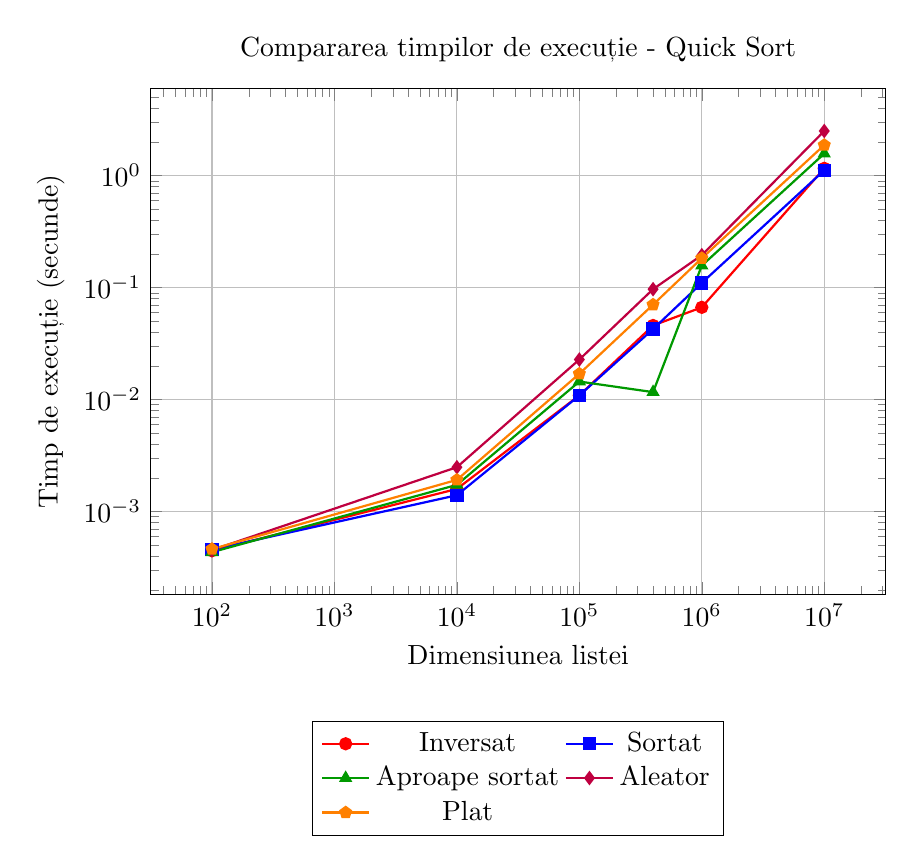
\begin{tikzpicture}
\begin{axis}[
    title={Compararea timpilor de execuție - Quick Sort},
    xlabel={Dimensiunea listei},
    ylabel={Timp de execuție (secunde)},
    xmode=log,
    ymode=log,
    log basis x=10,
    log basis y=10,
    grid=major,
    minor grid style={gray!20},
    major grid style={gray!50},
    width=0.9\textwidth,
    height=8cm,
    legend style={at={(0.5,-0.25)}, anchor=north, legend columns=2}
]

\addplot[color=red, mark=*, thick] coordinates {
    (100,0.000446884)
    (10000,0.00159377)
    (100000,0.0109133)
    (400000,0.0459573)
    (1000000,0.0667528)
    (10000000,1.16346)
};
\addlegendentry{Inversat}

\addplot[color=blue, mark=square*, thick] coordinates {
    (100,0.000457227)
    (10000,0.00140048)
    (100000,0.0108926)
    (400000,0.0426855)
    (1000000,0.11028)
    (10000000,1.11758)
};
\addlegendentry{Sortat}

\addplot[color=green!60!black, mark=triangle*, thick] coordinates {
    (100,0.000434371)
    (10000,0.00173346)
    (100000,0.0145072)
    (400000,0.0116722)
    (1000000,0.157436)
    (10000000,1.5754)
};
\addlegendentry{Aproape sortat}

\addplot[color=purple, mark=diamond*, thick] coordinates {
    (100,0.000453481)
    (10000,0.00249213)
    (100000,0.0228065)
    (400000,0.0969445)
    (1000000,0.195177)
    (10000000,2.5079)
};
\addlegendentry{Aleator}

\addplot[color=orange, mark=pentagon*, thick] coordinates {
    (100,0.000462744)
    (10000,0.00192068)
    (100000,0.0170093)
    (400000,0.0705046)
    (1000000,0.18327)
    (10000000,1.87794)
};
\addlegendentry{Plat}

\end{axis}
\end{tikzpicture}
\caption{Compararea timpilor de execuție pentru Quick Sort, în funcție de tipul și dimensiunea listei}
\label{fig:quick-loglog}
\end{figure}

\paragraph*{Observații:}
\begin{itemize}
    \item Pentru listele aleatorii, timpul de execuție a urmat comportamentul așteptat, crescând aproximativ proporțional cu $n\log n$.
    \item Listele aproape sortate și sortate au avut timpi de execuție puțin mai mari decât listele aleatorii, ceea ce sugerează un ușor impact negativ al alegerii pivotului fix.
    \item În cazul listelor invers sortate, timpul de execuție a fost relativ apropiat de cel pentru date aleatorii, dar s-au observat ușoare creșteri, confirmând teoria despre cazurile proaste la Quick Sort \cite{bigocheatsheet}.
    \item Se poate remarca o anomalie minoră pentru listele aproape sortate, unde timpul pentru $n=400.000$ a fost mult mai mic decât așteptat. Această scădere neașteptată se explică prin faptul că, uneori, datele aproape ordonate pot duce la partitionări foarte eficiente chiar și fără pivot aleatoriu.
    \item În implementări comerciale sau optimizate (de exemplu în biblioteca C++ STL), Quick Sort folosește tehnici suplimentare precum "median of three" sau randomizare pentru alegerea pivotului, tocmai pentru a evita aceste riscuri \cite{cppreferenceqsort}.
\end{itemize}


\subsubsection{Rezultate pentru Merge Sort}

Merge Sort este un algoritm stabil, bazat pe tehnica divide-et-impera, cu complexitate garantată $\mathcal{O}(n\log n)$ în toate cazurile. Deoarece necesită spațiu auxiliar proporțional cu dimensiunea listei, era de așteptat ca timpul de execuție să fie ușor influențat de alocările de memorie, mai ales pe liste foarte mari.

\begin{table}[H]
\centering
\begin{tabular}{|l|c|c|c|c|c|c|}
\hline
\textbf{Tip listă} & \textbf{100} & \textbf{10.000} & \textbf{100.000} & \textbf{400.000} & \textbf{1.000.000} & \textbf{10.000.000} \\
\hline
Inversat & 0.000454368 & 0.00196091 & 0.0199178 & 0.0798976 & 0.200191 & 2.25947 \\
\hline
Sortat & 0.00185973 & 0.00193904 & 0.0180503 & 0.0787589 & 0.203933 & 2.41023 \\
\hline
Aproape sortat & 0.000391713 & 0.00215365 & 0.0201851 & 0.0864965 & 0.223203 & 2.58547 \\
\hline
Aleator & 0.000475315 & 0.00291285 & 0.0278087 & 0.116938 & 0.314855 & 3.48368 \\
\hline
Plat & 0.000387329 & 0.00232341 & 0.0221688 & 0.0930226 & 0.245374 & 2.68084 \\
\hline
\end{tabular}
\caption{Timpul mediu de execuție pentru Merge Sort, în funcție de tipul și dimensiunea listei}
\label{tab:rezultate-merge}
\end{table}

\begin{figure}[H]
\centering
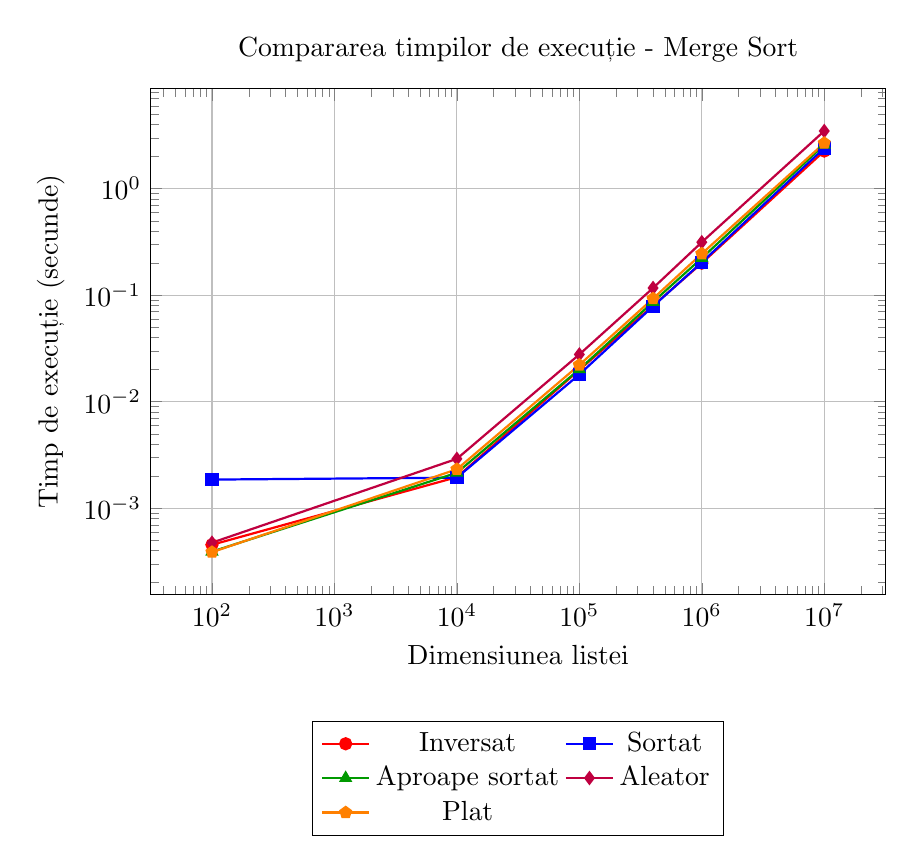
\begin{tikzpicture}
\begin{axis}[
    title={Compararea timpilor de execuție - Merge Sort},
    xlabel={Dimensiunea listei},
    ylabel={Timp de execuție (secunde)},
    xmode=log,
    ymode=log,
    log basis x=10,
    log basis y=10,
    grid=major,
    minor grid style={gray!20},
    major grid style={gray!50},
    width=0.9\textwidth,
    height=8cm,
    legend style={at={(0.5,-0.25)}, anchor=north, legend columns=2}
]

\addplot[color=red, mark=*, thick] coordinates {
    (100,0.000454368)
    (10000,0.00196091)
    (100000,0.0199178)
    (400000,0.0798976)
    (1000000,0.200191)
    (10000000,2.25947)
};
\addlegendentry{Inversat}

\addplot[color=blue, mark=square*, thick] coordinates {
    (100,0.00185973)
    (10000,0.00193904)
    (100000,0.0180503)
    (400000,0.0787589)
    (1000000,0.203933)
    (10000000,2.41023)
};
\addlegendentry{Sortat}

\addplot[color=green!60!black, mark=triangle*, thick] coordinates {
    (100,0.000391713)
    (10000,0.00215365)
    (100000,0.0201851)
    (400000,0.0864965)
    (1000000,0.223203)
    (10000000,2.58547)
};
\addlegendentry{Aproape sortat}

\addplot[color=purple, mark=diamond*, thick] coordinates {
    (100,0.000475315)
    (10000,0.00291285)
    (100000,0.0278087)
    (400000,0.116938)
    (1000000,0.314855)
    (10000000,3.48368)
};
\addlegendentry{Aleator}

\addplot[color=orange, mark=pentagon*, thick] coordinates {
    (100,0.000387329)
    (10000,0.00232341)
    (100000,0.0221688)
    (400000,0.0930226)
    (1000000,0.245374)
    (10000000,2.68084)
};
\addlegendentry{Plat}

\end{axis}
\end{tikzpicture}
\caption{Compararea timpilor de execuție pentru Merge Sort, în funcție de tipul și dimensiunea listei}
\label{fig:merge-loglog}
\end{figure}

\paragraph{Observații:}
\begin{itemize}
    \item Timpul de execuție crește constant cu dimensiunea listei, așa cum era de așteptat pentru un algoritm de complexitate $\mathcal{O}(n \log n)$ \cite{bigocheatsheet}.
    \item Nu apar diferențe semnificative între tipurile de liste, ceea ce confirmă că Merge Sort este stabil indiferent de ordonarea inițială a datelor.
    \item Pentru dimensiunile mici (100, 10.000), lista sortată a avut un timp ușor mai mare, posibil din cauza mecanismului de recursivitate care nu aduce beneficii speciale pentru date deja ordonate.
    \item Nu au fost observate anomalii majore sau scăderi de performanță pe niciun caz de testare.
\end{itemize}

\subsection{Comparație directă a performanțelor medii ale algoritmilor}

Pentru o imagine generală și practică a performanței algoritmilor analizați, am calculat timpii medii de execuție pentru fiecare algoritm pe toate tipurile de liste testate (inversate, sortate, aproape sortate, aleatoare și plate), pentru dimensiuni variabile.


\begin{table}[H]
\centering
\begin{tabular}{|l|c|c|c|c|c|c|}
\hline
\textbf{Algoritm}     & \textbf{100}   & \textbf{10\,000} & \textbf{100\,000} & \textbf{400\,000} & \textbf{1\,000\,000} & \textbf{10\,000\,000} \\
\hline
Bubble Sort           & 0.00049        & 0.34689          & 34.41789          & --                & --                  & --                   \\
Selection Sort        & 0.00044        & 0.18256          & 18.47828          & --                & --                  & --                   \\
Insertion Sort        & 0.00052        & 0.08405          & 8.34072           & --                & --                  & --                   \\
Merge Sort            & 0.00071        & 0.00226          & 0.02163           & 0.09102           & 0.23751             & 2.68393              \\
Quick Sort            & 0.00045        & 0.00183          & 0.01523           & 0.05355           & 0.14258             & 1.64846              \\
Heap Sort             & 0.00045        & 0.00476          & 0.04178           & 0.20071           & 0.56365             & 7.23896              \\
\hline
\end{tabular}
\caption{Compararea performanței medii (în secunde) a algoritmilor de sortare, în funcție de dimensiunea listei}
\label{tab:comparare-medii}
\end{table}

\begin{figure}[H]
\centering
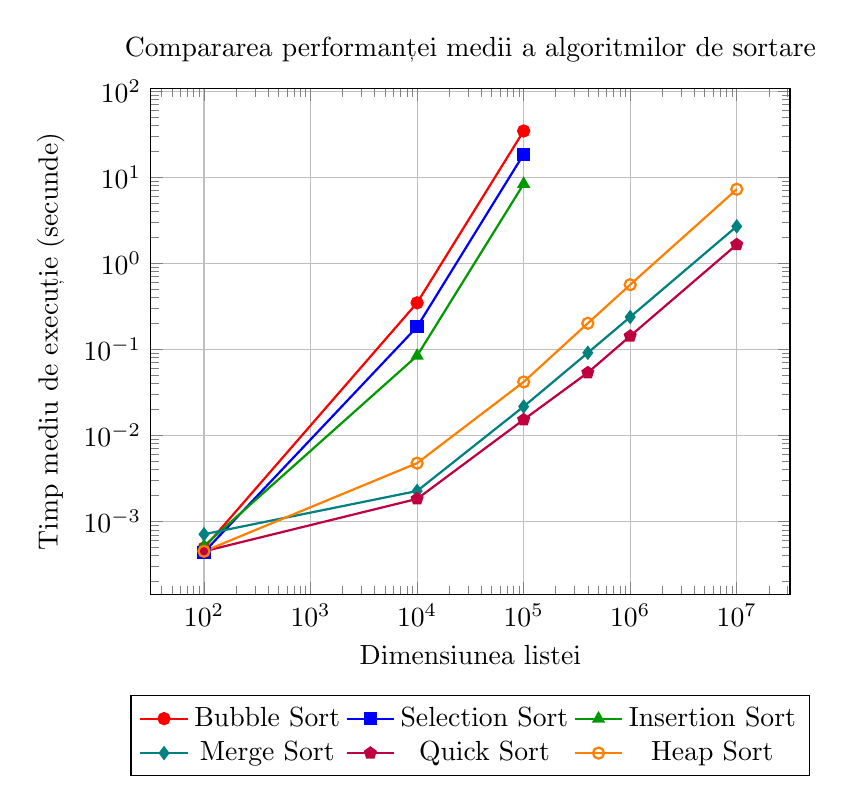
\begin{tikzpicture}
\begin{axis}[
    title={Compararea performanței medii a algoritmilor de sortare},
    xlabel={Dimensiunea listei},
    ylabel={Timp mediu de execuție (secunde)},
    xmode=log, ymode=log,
    log basis x=10, log basis y=10,
    grid=major,
    width=0.8\textwidth,
    height=8cm,
    legend style={at={(0.5,-0.2)},anchor=north,legend columns=3}
]
\addplot[color=red, mark=*, thick] coordinates {
    (100,0.00049)
    (10000,0.34689)
    (100000,34.41789)
};
\addlegendentry{Bubble Sort}

\addplot[color=blue, mark=square*, thick] coordinates {
    (100,0.00044)
    (10000,0.18256)
    (100000,18.47828)
};
\addlegendentry{Selection Sort}

\addplot[color=green!60!black, mark=triangle*, thick] coordinates {
    (100,0.00052)
    (10000,0.08405)
    (100000,8.34072)
};
\addlegendentry{Insertion Sort}

\addplot[color=teal, mark=diamond*, thick] coordinates {
    (100,0.00071)
    (10000,0.00226)
    (100000,0.02163)
    (400000,0.09102)
    (1000000,0.23751)
    (10000000,2.68393)
};
\addlegendentry{Merge Sort}

\addplot[color=purple, mark=pentagon*, thick] coordinates {
    (100,0.00045)
    (10000,0.00183)
    (100000,0.01523)
    (400000,0.05355)
    (1000000,0.14258)
    (10000000,1.64846)
};
\addlegendentry{Quick Sort}

\addplot[color=orange, mark=o, thick] coordinates {
    (100,0.00045)
    (10000,0.00476)
    (100000,0.04178)
    (400000,0.20071)
    (1000000,0.56365)
    (10000000,7.23896)
};
\addlegendentry{Heap Sort}

\end{axis}
\end{tikzpicture}
\caption{Graficul comparativ al timpilor medii de execuție pentru cei șase algoritmi, în funcție de dimensiunea listei}
\label{fig:comparare-medii-grafic}
\end{figure}


\textbf{Observații:}

\begin{itemize}
\item \textbf{Bubble Sort}, \textbf{Selection Sort} și \textbf{Insertion Sort}, algoritmi de complexitate $O(n^2)$, sunt eficienți numai pentru liste mici (până la 10.000 de elemente), iar pentru dimensiuni mai mari, timpul de execuție crește exponențial.
\item Pentru liste mici (100 elemente), diferențele între algoritmi sunt neglijabile și nu indică clar superioritatea unui algoritm.

\item Începând de la 10.000 elemente, \textbf{Merge Sort}, \textbf{Quick Sort} și \textbf{Heap Sort}, cu complexitate $O(n \log n)$, prezintă timpi mult mai mici, confirmând superioritatea clară față de algoritmii $O(n^2)$.

\item \textbf{Quick Sort} a demonstrat cel mai bun timp mediu global dintre algoritmii $O(n \log n)$, fiind cel mai rapid pe toate seturile mari de date testate. Acest comportament este tipic implementărilor optimizate ale acestui algoritm.

\item Deși \textbf{Heap Sort} a fost consistent ca performanță, acesta a fost, în medie, mai lent decât \textbf{Quick Sort} și \textbf{Merge Sort}, probabil datorită costului operațiilor de menținere a structurii heap.

\item Rezultatele experimentale sunt în concordanță cu teoria complexităților algoritmilor, confirmând că algoritmii $O(n \log n)$ sunt preferabili pentru aplicații practice care manipulează volume mari de date.
\end{itemize}

Această analiză evidențiază clar avantajele utilizării algoritmilor cu complexitate $O(n \log n)$ în contexte reale, în special când se lucrează cu date voluminoase, și subliniază importanța alegerii adecvate a algoritmului în funcție de contextul specific aplicației.



%====================================================================
\section{Interpretarea rezultatelor}
%====================================================================
\begin{itemize}
    \item Rezultatele confirmă complexitățile așteptate, cu diferențe clare între algoritmii $\mathcal{O}(n^2)$ și $\mathcal{O}(n\log n)$.
    \item Heap Sort și Merge Sort au prezentat variații minore, iar Quick Sort a avut degradări pe liste aproape sortate.
    \item Optimizările STL, cache-ul procesorului și distribuția datelor au influențat timpii măsurați.
    \item Testele au fost efectuate în condiții controlate, cu seturi de date generate automat și fără aplicații concurente.
    \item Dintre algoritmii $\mathcal{O}(n\log n)$, Quick Sort a avut cel mai mic timp mediu pe majoritatea dimensiunilor, urmat de Merge Sort şi apoi de Heap Sort, ceea ce reflectă costurile suplimentare de întreţinere a heap‑ului.
    \item Pe dimensiuni foarte mici (100–1000 elemente), diferenţele de performanţă sunt neglijabile, însă de la 10000 de elemente în sus timpii celor trei algoritmi $\mathcal{O}(n^2)$ cresc foarte mult, în timp ce Quick, Merge şi Heap rămân eficienţi.
    \item Graficul comparativ arată clar că timpii algoritmilor cu complexitate $\mathcal{O}(n^2)$ cresc foarte rapid pe măsură ce numărul de elemente creşte, în timp ce timpii algoritmilor $\mathcal{O}(n\log n)$ cresc mult mai lent, ceea ce îi face mult mai potriviţi pentru seturi mari de date.
\end{itemize}


%====================================================================
\section{Concluzii}
%====================================================================
Lucrarea a comparat teoretic și experimental șase algoritmi de sortare. Rezultatele obținute au confirmat în mare parte așteptările teoretice și au evidențiat situațiile în care performanța practică diferă.

\subsection{Rezumatul lucrării}
\begin{itemize}
    \item Algoritmii cu complexitate $\mathcal{O}(n^2)$ (Bubble Sort, Selection Sort, Insertion Sort) au funcționat bine doar pe liste mici sau aproape ordonate.
    \item Algoritmii cu complexitate $\mathcal{O}(n\log n)$ (Merge Sort, Quick Sort, Heap Sort) au fost mult mai eficienți pe liste mari.
    \item Quick Sort a avut degradări pe liste aproape sortate din cauza alegerii pivotului fix.
    \item Heap Sort, bazat pe funcțiile STL, a avut un comportament constant, cu variații minore în unele cazuri.
\end{itemize}

\subsection{Perspective și îmbunătățiri posibile}
\begin{itemize}
    \item Extinderea experimentelor pentru liste de dimensiuni mai mari (peste $10^7$ elemente).
    \item Introducerea algoritmilor moderni precum Timsort sau Radix Sort pentru comparații suplimentare.
    \item Analiza detaliată a consumului de memorie și a impactului caching-ului procesorului asupra performanțelor.
    \item Implementarea unor variante optimizate ale algoritmilor existenți, de exemplu Quick Sort cu pivot randomizat.
\end{itemize}


%--------------------------------------------------------------------
\section*{Referințe bibliografice}
%--------------------------------------------------------------------
\begin{thebibliography}{9}
\bibitem{bigocheatsheet}
  Eric Rowell,
  \textit{Big‑O Algorithm Complexity Cheat Sheet},
  disponibil online la \url{https://www.bigocheatsheet.com/},
  accesat în 5 aprilie 2025.

\bibitem{mit_insertion}
  Massachusetts Institute of Technology (MIT),
  \textit{Introduction to Algorithms, Lecture Notes 6.006 - Insertion Sort},
  disponibil online la \url{https://ocw.mit.edu/courses/electrical-engineering-and-computer-science/6-006-introduction-to-algorithms-fall-2011/readings/lecture-notes/MIT6_006F11_Lec01.pdf},
  accesat în 10 aprilie 2025.

\bibitem{wiki_bubble}
  Wikipedia,
  \textit{Bubble Sort},
  disponibil online la \url{https://en.wikipedia.org/wiki/Bubble_sort},
  accesat în 20 aprilie 2025.

\bibitem{wiki_merge}
  Wikipedia,
  \textit{Merge Sort},
  disponibil online la \url{https://en.wikipedia.org/wiki/Merge_sort},
  accesat în 20 aprilie 2025.

\bibitem{wiki_quick}
  Wikipedia,
  \textit{Quick Sort},
  disponibil online la \url{https://en.wikipedia.org/wiki/Quicksort},
  accesat în 20 aprilie 2025..

\bibitem{wiki_heap}
  Wikipedia,
  \textit{Heap Sort},
  disponibil online la \url{https://en.wikipedia.org/wiki/Heapsort},
  accesat în 10 mai 2025.

\bibitem{cppreferenceheap}
  cppreference.com,
  \textit{std::make\_heap, std::pop\_heap, std::sort\_heap},
  disponibil online la \url{https://en.cppreference.com/w/cpp/algorithm/make_heap},
  accesat în 10 mai 2025.

\bibitem{cppreferenceqsort}
  cppreference.com,
  \textit{std::sort - Implementation Notes},
  disponibil online la \url{https://en.cppreference.com/w/cpp/algorithm/sort},
  accesat în 10 mai 2025.

\end{thebibliography}


\newpage

%--------------------------------------------------------------------
\appendix
\section*{Anexe}
%--------------------------------------------------------------------
\addcontentsline{toc}{section}{Anexe}

\subsection*{Anexa A – Cod sursă algoritmi de sortare utilizați}

\subsubsection*{Bubble Sort}
Mai jos avem implementarea folosita pentru bubble sort.

\begin{lstlisting}[language=C++, caption={Bubble Sort}, label={lst:bubble}]
void bubble_sort(Vec& vector) {
    // parcurgem fiecare pozitie pentru a muta valorile mari spre final
    for (size_t i = 0; i + 1 < vector.size(); ++i) {
        bool schimbare = false;

        // comparam elemente adiacente si le interschimbam daca sunt in ordine gresita
        for (size_t j = 0; j + 1 < vector.size() - i; ++j) {
            if (vector[j] > vector[j + 1]) {
                std::swap(vector[j], vector[j + 1]);
                schimbare = true;
            }
        }

        // daca in aceasta trecere prin bucla nu s-a facut nicio schimbare, vectorul este sortat
        if (!schimbare) break;
    }
}
\end{lstlisting}

\subsubsection*{Heap Sort}

Mai jos este implementarea folosită pentru Heap Sort, care utilizează funcțiile standard \texttt{std::make\_heap} și \texttt{std::sort\_heap} din biblioteca STL.

\begin{lstlisting}[language=C++, caption={Heap Sort}, label={lst:heap}]
void heap_sort(Vec& vector) {
    // transforma vectorul intr-un heap max
    std::make_heap(vector.begin(), vector.end());
    // sorteaza vectorul folosind proprietatea de heap
    std::sort_heap(vector.begin(), vector.end());
}

\end{lstlisting}


\subsubsection*{Selection Sort}

Algoritmul de selecție a fost implementat simplu, urmărind alegerea minimului la fiecare pas.

\begin{lstlisting}[language=C++, caption={Selection Sort}, label={lst:selection}]
void selection_sort(Vec& vector) {
    // pentru fiecare pozitie cauta minimul si il muta pe pozitia curenta
    for (size_t i = 0; i + 1 < vector.size(); ++i) {
        size_t minim = i;
        for (size_t j = i + 1; j < vector.size(); ++j) {
            if (vector[j] < vector[minim])
                minim = j;
        }
        std::swap(vector[i], vector[minim]);
    }
}
\end{lstlisting}

\textbf{Observații}: Algoritmul efectuează întotdeauna același număr de comparații, indiferent de ordonarea inițială a datelor.

\vspace{0.5cm}

\subsubsection*{Insertion Sort}

Sortarea prin inserție introduce fiecare element la locul potrivit în secțiunea deja ordonată.

\begin{lstlisting}[language=C++, caption={Insertion Sort}, label={lst:insertion}]
void insertion_sort(Vec& vector) {
    // insereaza fiecare element pe pozitia corecta in partea sortata
    for (size_t i = 1; i < vector.size(); ++i) {
        long long element_curent = vector[i];
        size_t j = i;
        while (j > 0 && vector[j - 1] > element_curent) {
            vector[j] = vector[j - 1];
            --j;
        }
        vector[j] = element_curent;
    }
}
\end{lstlisting}

\textbf{Observații}: În caz de liste aproape sortate, inserția devine extrem de rapidă, cu un număr minim de mutări.

\vspace{0.5cm}
\clearpage

\subsubsection*{Merge Sort}

Algoritmul de interclasare este implementat recursiv, folosind un vector auxiliar.

\begin{lstlisting}[language=C++, caption={Merge Sort}, label={lst:merge}]
void interclasare_recursiva(Vec& vector, Vec& temporar, size_t stanga, size_t dreapta) {
    // daca segmentul are maxim un element, este deja sortat
    if (dreapta - stanga <= 1) return;
    
    size_t mijloc = (stanga + dreapta) / 2;
    
    // sorteaza recursiv cele doua jumatati
    interclasare_recursiva(vector, temporar, stanga, mijloc);
    interclasare_recursiva(vector, temporar, mijloc, dreapta);

    // interclaseaza cele doua jumatati sortate
    size_t i = stanga, j = mijloc, k = stanga;
    while (i < mijloc && j < dreapta)
        temporar[k++] = (vector[i] <= vector[j]) ? vector[i++] : vector[j++];
    while (i < mijloc) temporar[k++] = vector[i++];
    while (j < dreapta) temporar[k++] = vector[j++];

    // copiaza inapoi in vectorul initial
    for (size_t p = stanga; p < dreapta; ++p)
        vector[p] = temporar[p];
}

void merge_sort(Vec& vector) {
    // aloca vector temporar si incepe sortarea
    Vec temporar(vector.size());
    interclasare_recursiva(vector, temporar, 0, vector.size());
}

\end{lstlisting}

\textbf{Observații}: Metoda necesită memorie suplimentară, dar garantează un timp de rulare optim pentru orice caz.

\newpage

\subsubsection*{Quick Sort}

Sortarea rapidă a fost implementată recursiv, cu alegerea pivotului în mijloc.

\begin{lstlisting}[language=C++, caption={Quick Sort}, label={lst:quick}]
void recursiveQS(Vec& vector, size_t stanga, size_t dreapta) {
    // daca segmentul este invalid sau de dimensiune 0/1, nu se sorteaza
    if (stanga >= dreapta) return;

    // alegere pivot ca mediana
    long long pivot = vector[(stanga + dreapta) / 2];
    size_t i = stanga, j = dreapta;

    // partitionare in jurul pivotului
    while (i <= j) {
        while (vector[i] < pivot) ++i;
        while (vector[j] > pivot) --j;
        if (i <= j) {
            std::swap(vector[i], vector[j]);
            ++i;
            if (j > 0) --j;
        }
    }

    // apel recursiv pentru subsecvente
    if (stanga < j) recursiveQS(vector, stanga, j);
    if (i < dreapta) recursiveQS(vector, i, dreapta);
}

void quickSort(Vec& vector) {
    if (!vector.empty())
        recursiveQS(vector, 0, vector.size() - 1);
}

\end{lstlisting}

\textbf{Observații}: Pivotul ales ca mediană tinde să ofere o performanță apropiată de cea optimă, însă listele deja sortate pot genera cazuri defavorabile.

\clearpage

\subsection*{Anexa B – Codul sursa al programului care a generat listele}
\begin{lstlisting}[language=Python, caption={Generatorul de liste}, label={lst:gen}]
import os, numpy as np, gc

# dimensiunile listelor de generat
dimensiuni = [100, 10_000, 100_000, 400_000, 1_000_000, 10_000_000]

# tipurile de liste cerute
tipuri = ["aleator", "sortat", "inversat", "aproape_sortat", "plat"]

# directorul unde vom scrie fisierele CSV
os.makedirs("liste", exist_ok=True)

# --- generatoare pentru fiecare tip ---

def aleator(n):
    # valori intregi aleatoare in intervalul [0, 1e9)
    return np.random.randint(0, 1_000_000_000, n, np.int64)

def sortat(n):
    # sir crescator 0, 1, 2, ...
    return np.arange(n, dtype=np.int64)

def inversat(n):
    # sir descrescator n-1, n-2, ...
    return np.arange(n - 1, -1, -1, dtype=np.int64)

def aproape_sortat(n, p=0.05):
    # lista sortata cu p*100% pozitii incurcate
    a = np.arange(n, dtype=np.int64)
    k = int(n * p)
    if k:  # doar daca avem ce schimba
        i1 = np.random.choice(n, k, False)  # pozitii unice
        i2 = np.random.choice(n, k, True)   # pozitii (posibil) repetate
        a[i1], a[i2] = a[i2], a[i1]
    return a

def plat(n, distincte=20):
    # lista lunga cu putine valori distincte
    return np.random.choice(distincte, n).astype(np.int64)

# dictionar pentru acces rapid
gen = {
    "aleator": aleator,
    "sortat": sortat,
    "inversat": inversat,
    "aproape_sortat": aproape_sortat,
    "plat": plat,
}

for tip in tipuri:
    for n in dimensiuni:
        date = gen[tip](n)
        nume_fisier = f"liste/{tip}_{n}.csv"
        with open(nume_fisier, "w") as f:
            # scriem ca o singura coloana, un numar pe linie
            date.tofile(f, sep="\n", format="%d")
        # eliberam memoria pentru dimensiuni mari
        del date
        gc.collect()
\end{lstlisting}

\subsection*{Anexa C – Github}
Datele in format raw, impreuna cu rezultatele complete si codul sursa sunt disponibile pe Github la 
\href{https://github.com/DavidGavrilescu/MPI}{DavidGavrilescu/MPI}

%----------------------------------------------------------------------
\end{document}